% Modified from https://github.com/PetarV-/TikZ/blob/master/Graph%20convolution/graph_convolution.tex

\documentclass[crop, tikz]{standalone}
\usepackage{tikz}

\usetikzlibrary{arrows,shapes, matrix}

% \definecolor{mygreen}{rgb}{0,0.6,0}
\usepackage{xcolor}
% \colorlet{LightCyan}{cyan!30}
% \colorlet{LightGray}{lightgray!30}

\pgfdeclarelayer{background}
\pgfsetlayers{background,main}

\tikzstyle{vertex}=[circle,fill=black!25,minimum size=20pt,inner sep=0pt]
\tikzstyle{selected vertex} = [vertex, fill=red!34]
\tikzstyle{select vertex} = [vertex, fill=cyan]
\tikzstyle{selectx vertex} = [vertex, fill=green!24]
\tikzstyle{edge} = [draw,thick,-]
\tikzstyle{selected edge} = [draw,line width=5pt,-,red!50]

% \tikzset{matrix of node keys/.code={
% 	\matrix (emb_b) [right=of b, matrix of nodes,row sep=-\pgflinewidth, nodes={draw}]
% 	{
% 		|[fill=red!20]| 1 & |[fill=red!25]| 0 & |[fill=red!30]| 0 & |[fill=red!35]| 0\\
% 	};
% }}

\begin{document}

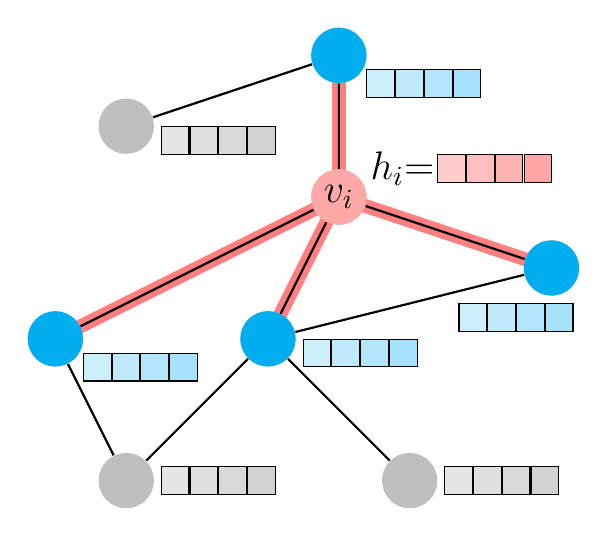
\begin{tikzpicture}[scale=1.8, auto,swap]
    % Nodes
    \foreach \pos/\name in {{(2,2)/a}, {(2,1)/b}, {(3.5,0.5)/c}, {(0.5,1.5)/h},
                            {(0,0)/d}, {(1.5,0)/e}, {(0.5,-1)/f}, {(2.5,-1)/g}}
        \node[vertex] (\name) at \pos {};

    % Red node
    \foreach \vertex / \fr in {b/4}
        \path node[selected vertex] at (\vertex) {\Large $v_i$};

    % Blue nodes
    \foreach \vertex / \fr in {a/4, c/4, d/4, e/5}
        \path node[select vertex] at (\vertex) {}; % $h_{\vertex}$

    % Link creation
    \foreach \source/ \dest /\weight in {b/a/7, c/b/8, d/b/9,
                                         e/b/7, e/c/5, a/h/9,
                                         f/d/6, f/e/8, g/e/9}
    \path[edge] (\source) -- (\dest);

    % Highlight links as red
    \begin{pgfonlayer}{background}
        \foreach \source / \dest in {b/c,d/b,a/b,b/e}
            \path[selected edge] (\source.center) -- (\dest.center);
    \end{pgfonlayer}
    
    % Red Embedding
	\matrix (emb_b) [matrix of nodes, minimum size=10pt, nodes={draw}] at (3.1, 1.2) { |[fill=red!20]| & |[fill=red!25]| & |[fill=red!30]| & |[fill=red!35]| \\ };
	\node[] (h_emb) at (2.45, 1.2) {\Large $h_i$=};
	
	% Blue Embeddings
	\matrix (emb_a) [matrix of nodes, minimum size=10pt, nodes={draw}] at (2.6, 1.8) { |[fill=cyan!20]| & |[fill=cyan!25]| & |[fill=cyan!30]| & |[fill=cyan!35]| \\ };
	\matrix (emb_c) [matrix of nodes, minimum size=10pt, nodes={draw}] at (3.25, 0.15) { |[fill=cyan!20]| & |[fill=cyan!25]| & |[fill=cyan!30]| & |[fill=cyan!35]| \\ };
	\matrix (emb_d) [matrix of nodes, minimum size=10pt, nodes={draw}] at (0.6, -0.2) { |[fill=cyan!20]| & |[fill=cyan!25]| & |[fill=cyan!30]| & |[fill=cyan!35]| \\ };
	\matrix (emb_e) [matrix of nodes, minimum size=10pt, nodes={draw}] at (2.15, -0.1) { |[fill=cyan!20]| & |[fill=cyan!25]| & |[fill=cyan!30]| & |[fill=cyan!35]| \\ };

	% Grey Embeddings
	\matrix (emb_f) [matrix of nodes, minimum size=10pt, nodes={draw}] at (1.15, -1) { |[fill=gray!20]| & |[fill=gray!25]| & |[fill=gray!30]| & |[fill=gray!35]| \\ };
	\matrix (emb_g) [matrix of nodes, minimum size=10pt, nodes={draw}] at (3.15, -1) { |[fill=gray!20]| & |[fill=gray!25]| & |[fill=gray!30]| & |[fill=gray!35]| \\ };
	\matrix (emb_h) [matrix of nodes, minimum size=10pt, nodes={draw}] at (1.15, 1.4) { |[fill=gray!20]| & |[fill=gray!25]| & |[fill=gray!30]| & |[fill=gray!35]| \\ };

\end{tikzpicture}

\end{document}